\chapter{Experiments} \label{chapterexperiments}
In this chapter we describe experiments and their results for our implementation of all algorithms described in the previous chapter.
For testing performance of algorithms we have implemented data set generator which provide wide variety of configuration options of generating the data.

\section{Data set generator}
When we want to generate $n$ observations without outliers that satisfies linear regression model we can do it as follows:

\begin{algo}[Generate clean data] \label{generate:linear:model}
    \mbox{}\vspace{\dimexpr-\baselineskip-\topsep}
\\
    \begin{enumerate}
        \item Generate regression coefficients $\vec{w} = (w_1, \ldots, w_p)$ and set $\sigma^{2}$.
        \item Generate explanatory variable $\vec{x_i}$.
        \item Generate random noise $\varepsilon_i \sim \mathcal{N}(0,\,\sigma^{2})$.
        \item Simulate dependent variable $y_i = \vec{w}^T\vec{x_i} + \varepsilon_i$.
        \item Repeat steps $2$--$4$ $n$ times.
    \end{enumerate}
\end{algo}
As a result we obtain $\vec{X}$ and $\vec{y}$. Regression coefficients can be set to arbitrary values, but if we do not want to have dummy explanatory variables, then they are supposed to be non-zero. All $\vec{x_i}$ should be generated independently and it is very common that we generate all $\vec{x_i}$ from normal distribution. 

Another thing that needs to be considered is the intercept. In this work we assumed that our data already include intercept, so in that case $w_1$ is equal to intercept and all $x_{i_1}$ should be equal to $1$. Note that same result can be obtained by generating data without intercept and with $\varepsilon_i \sim \mathcal{N}(\mu,\,\sigma^{2})$. We can then extend matrix $\vec{X}$ so that we add first column that contains only $1$s. This approach is very common and software for estimating regression coefficients usually allows to set parameter which determines if intercept should be used; if so, the column of $1$s is added. For that reason we generate our data sets using this approach. That means we generate $\varepsilon_i \sim \mathcal{N}(\mu,\,\sigma^{2})$ and column of $1$s is included only in case we set parameter for using intercept when fitting the data set. 

\subsection{Generating outliers}
As we have already described in Section~\ref{outliers:info} we can describe different types of the outliers: vertical outliers and two types leverage points --- good leverage points and bad leverage points. Those types of outliers are visualized on Figure~\ref{outliers:types:figure}. We can see that good leverage points are not deemed as an outliers here, even if they are distant observations, because they follow the linear pattern. 

\begin{figure}[h]
    \centering
    
% even more fun
\begin{tikzpicture}
    \begin{axis}[
        xlabel={$\vec{x}$},
        ylabel={$y$},
        xmin=0,
        xmax=5,
        ymin=0,
        ymax=7,
        xtick = {0},
        ytick = {0}, 
        domain = 0:8,
        axis lines = middle,
        clip=false
      ]
    
      % VERTICAL OUTLIERS
      \addplot[soldot, red]coordinates {(1.25,5.25*0.8+0.85)} node [anchor=north west,text=black] {Vertical outliers};
      \addplot[soldot, red]coordinates {(1.2,5.4*0.8+0.95)} node [anchor=north east,text=black] {};
      \addplot[soldot, red]coordinates {(1.35,5.4*0.8+1.1)} node [anchor=north east,text=black] {};


      % REGULAR OBSERVATIONS
      \addplot[soldot,black]coordinates {(2.45, 2.45*0.8+0.94)} node [anchor=north east,text=black] {};
      \addplot[soldot,black]coordinates {(2.2, 2.3*0.8+1.12)} node [anchor=north east,text=black] {};
      \addplot[soldot,black]coordinates {(2.1, 2.1*0.8+0.8)} node [anchor=north west,text=black] {Regular observations};
      \addplot[soldot,black]coordinates {(2, 2*0.8+1.1)} node [anchor=north east,text=black] {};
      \addplot[soldot, black]coordinates {(1.7,1.7*0.8+1)} node [anchor=north east,text=black] {};
      \addplot[soldot, black]coordinates {(1.5,2.295)} node [anchor=north east,text=black] {};
      \addplot[soldot,black]coordinates {(0.8, 0.8*0.8+1.1)} node [anchor=north east,text=black] {};
      \addplot[soldot, black]coordinates {(1.25,1.25*0.8+0.8)} node [anchor=north east,text=black] {};
      \addplot[soldot, black]coordinates {(1.2,2.28)} node [anchor=north east,text=black] {};
      \addplot[soldot, black]coordinates {(0.6,1.4)} node [anchor=north east,text=black] {};
      \addplot[soldot, black]coordinates {(0.9,1.8)} node [anchor=north east,text=black] {};
      
      % GOOD LEVERAGE POINTS
      \addplot[soldot,black]coordinates {(5, 5*0.8+0.94)} node [anchor=north east,text=black] {};
      \addplot[soldot,black]coordinates {(4.8, 4.8*0.8+1.1)} node [anchor=north west,text=black] {Good leverage points};

      % BAD LEVERAGE POINTS
      \addplot[soldot,red]coordinates {(5.51, 0.5)} node [anchor=north east,text=black] {};
      \addplot[soldot,red]coordinates {(5.7, 0.6)} node [anchor=north west,text=black] {Bad leverage points};

      % plot of main model
      \addplot [domain=-1:6, samples=2, dashed] {0.8*x+1};      
    \end{axis} 
\end{tikzpicture}

    \caption{Different types of outliers.  }
    \label{outliers:types:figure}
\end{figure}

Moreover, the data set can contain multiple observations that satisfies linear regression model but with different regression coefficients. That means such data set can contain data from multiple different models.

To generate the vertical outliers we only need to modify step $3$ of Algorithm~\ref{generate:linear:model}. We have multiple options:
\begin{itemize}
    \item Generate $\varepsilon_i$ from $\mathcal{N}(\mu,\,\sigma^{2})$ but use different parameter  $\mu$ and $\sigma^{2}$ than which were used for generating regular observations.
    \item Generate $\varepsilon_i$ from some heavy tailed or asymmetrical distribution like  Log-normal or exponential distribution.
    \item Combine both above so that we randomly choose distribution and randomly generate parameters for such distribution.
\end{itemize}
The last option is the most versatile so we use this option. 

Because we generate $\vec{x_i}$ from the normal distribution, we can generate leverage points just by changing parameter $\mu$  of this distribution. If we consequently generate $\varepsilon_i$ from the same distribution with same parameters as for the regular observations, we obtain good leverage points. On the other hand if we generate $\varepsilon_i$ as described above, we obtain bad leverage points.

If we want to generate outliers that correspond to the different model we can just set the regression coefficients $\vec{w}$ differently. It is also possible to use different parameters of normal distribution for generating $\vec{x_i}$ and parameters for generating $\varepsilon_i$. Theoretically we are able to introduce outliers even into this model, but when this model is ``outlier'' by itself relative to the original model, it is not needed. By this approach we would be able to generate the observations from arbitrary number of differ models, but for the sake of the simplicity we introduce only one different model. 

\section{Data sets}
We have implemented ideas from previous section to the data set generator with following parameters:
\begin{itemize}
    \item $n$ and $p$ for setting number of the generated observations and dimension of the explanatory variables
    \item $outlier~ratio$ for setting proportion of the outliers in the data set. This include vertical outliers, bad leverage points and also outliers from the second model.
    \item $leverage~ratio$ proportion of the explanatory variables that are generated as leverage points.
    \item $\mu_{\vec{x}}, \sigma^{2}_{\vec{x}}$ parameters of the normal distribution for generating non outlying $\vec{x_i}$
    \item $\mu_{\vec{x_o}}, \sigma^{2}_{\vec{x_o}}$ parameters of the normal distribution for generating outlying $\vec{x_i}$ (leverage points)
    \item $\mu_{\varepsilon}, \sigma^{2}_{\varepsilon}$ parameters of the normal distribution for generating non outlying errors $\varepsilon_i$
    \item $\mu_{\varepsilon_o}, \sigma^{2}_{\varepsilon_o}$ parameters of the distribution for generating outlying errors $\varepsilon_i$. 
    \item $distrib_{\varepsilon_o}$ distribution from which outlying errors are generated --- options are normal distribution, log-normal distribution and exponential distribution (when exponential distribution is chosen, then only $\sigma^{2}_{\varepsilon_o}$ parameter is used)
    \item $2m~ratio$ proportion from the outliers which are generated from the second model
    \item $\mu_{\vec{x_{M2}}}, \sigma^{2}_{\vec{x_{M2}}}$ and $\mu_{\varepsilon_{M2}}, \sigma^{2}_{\varepsilon_{M2}}$ parameters for normal distributions for generating $\vec{x_i}$ and $\varepsilon_i$ respectively from the second model
\end{itemize}

We used this generator to generate three data sets $D1$, $D2$ and $D3$ which differ by the types of the outliers they contain:
\begin{itemize}
    \item $D1$ contains outliers which are not from the second model: vertical outliers, bad leverage points and good leverage points ($2m~ratio = 0$)
    \item $D2$ contains only outliers from the second model ($2m~ratio = 1$)
    \item $D3$ contain outliers of all described types. ($2m~ratio = 0.4$)
\end{itemize}

All three data sets are set to contain $20\%$ leverage points (thus $leverage~ratio = 0.2$) and non outlying $\vec{x_i}$ are generated from $\mathcal{N}(0,10)$ (thus $\mu_{\vec{x}} = 0, \sigma^{2}_{\vec{x}} = 10$). Other parameters are independently randomly generated from uniform distribution so that:
\begin{itemize}
    \item $\mu_{\vec{x_o}} \sim \mathcal{U}(20,\,60), \sigma^{2}_{\vec{x_o}} \sim \mathcal{U}(10,\,20)$
    \item $\mu_{\varepsilon} \sim \mathcal{U}(0,\,10), \sigma^{2}_{\varepsilon}  \sim \mathcal{U}(1,\,5)$ 
    \item $\mu_{\varepsilon_o} \sim \mathcal{U}(-50,\,50), \sigma^{2}_{\varepsilon_o} \sim \mathcal{U}(50,\,200)$
    \item $\mu_{\vec{x_{M2}}} \sim \mathcal{U}(-30,\,30), \sigma^{2}_{\vec{x_{M2}}} \sim \mathcal{U}(10,\,20)$
    \item  $\mu_{\varepsilon_{M2}}  \sim \mathcal{U}(-10,\,10) , \sigma^{2}_{\varepsilon_{M2}}\sim \mathcal{U}(1,\,5)$
    \item $distrib_{\varepsilon_o}$ is uniformly randomly set to normal, log-normal  or exponential distribution 
\end{itemize}
Finally parameters $n$, $p$ and $outlier~ratio$  are set depending on the experiment.

\section{Implementation of the algorithms}
We have implemented all described algorithms, moreover because algorithms for computing the feasible solution could be implemented both by calculating inversion and by calculating QR decomposition, we have implemented both version of those algorithms. Here is the list of all the implemented algorithm with their acronyms we use for labeling them:

\begin{description}
    \item[FAST-LTS] from Section~\ref{section_fast_lts} with all described improvements
    \item[FSA-I] from Section~\ref{section_feasible_solution}
    \item[FSA-QR] FSA using theory from Section~\ref{oeamoeammea}
    \item[MOEA-I] from Section~\ref{oeamoeammea} it is the improved version of OEA
    \item[MOEA-QR] MOEA using theory from Section~\ref{differentcomputation}
    \item[MMEA-I] from Section~\ref{mmeasection}
    \item[MMEA-QR] MMEA using theory from Section~\ref{differentcomputation}
    \item[BAB] from Section~\ref{sectionbab}
    \item[BSA] is the implementation of improved BAB (BSABAB) from Section~\ref{bsasection}
    \item[FAST-LTS-MMEA-I] combination of algorithms from Section~\ref{sectioncombined}
    \item[FAST-LTS-MOEA-I] another combination of algorithm from Section~\ref{sectioncombined}
    \item[MOEA-QR-BAB] BAB with sorting speedup as described in Section~\ref{sectionbab}
    \item[MOEA-QR-BSA] BSABAB using our idea from Section~\ref{bsasection}
    \item[P-BSA] probabilistic BSA using our idea from Section~\ref{bsasection}
\end{description}

These algorithms were first implemented in Python using the NumPy package~\cite{numpy}. The performance was low, so we have implemented all of the algorithms in \CC \ using the Eigen library~\cite{eigenweb} for matrix manipulation. On the other hand it is very popular today to use Python for data processing and manipulation; for that reason we have used pybind11 library~\cite{pybind11}, that exposes \CC \ types for Python and vice versa and written Python wrappers around the \CC \ implementation. 

Moreover pybind11 allows to bind Eigen types directly to the NumPy types (because both libraries are LAPACK compatible), so that it is possible to share pointers to the matrices between Eigen and NumPy so that the data does not have to be copied when transferring between Python an \CC.

That means that the data generator, all tests and experiments are implemented in Python; the \CC \  code is called only within the Python wrappers. It is also appropriate to mention that interface of the algorithms was created with regards to the popular scikit-learn package~\cite{scikit-learn}; the interface is almost identical, so all of the classes implementing the algorithms can be used in the same manner as classes from scikit-learn linear regression module.


\section{Results}
In two previous sections we have described our experimental setup. Here we report results of our experiments.

\subsection{Algorithms for finding the strong necessary condition}
In this section provide results of running multiple simulations, where we compare speed and accuracy of the algorithm finding subsets satisfying strong necessary condition e.g. $h$-element feasible subsets. For each combination parameters $n$, $p$ and $outlier~ratio$ ($out$) we generate data sets  $D1$, $D2$ and $D3$ $100$ times (each time new data sets are generated) and run all algorithms on those data sets. Value of $h$ is conservatively chosen so that $h = [(n/2] + [(p+1)/2]$. For all runs we use the intercept, so value $p$ represents dimension of $\vec{x}$ including intercept. All algorithm are set to run at most for $50$ steps and each of them is starting only from $1$ randomly selected $h$-element subset.  The results are given in Appendix [] in Tables~\ref{table1}, \ref{table2} and \ref{table3} for data sets $D1$, $D2$ and $D3$ respectively, were average CPU time from $100$ runs for each algorithm. We also measure cosine similarity and $L^2$ norm of a given solution compared to the regression coefficients given by the original model which does not contain outliers. For $n > 500$ cells for algorithm FSA-I and FSA-QR are empty. That is because times of the run of these algorithms were too slow and it would take weeks to finish all simulations.
At Figure~\ref{all_distances} are given box plots showing cosine similarity and $L^2$ norms of the results. 

As expected algorithms using QR decomposition provide slightly better results. Moreover the best results are given by the FSA-QR, because this algorithm does not use any equations for updating quantities and recalculate everything in the each step. On the other hand both FSA-I and FSA-QR are much slower because they does not use bounding condition as in the case MOEA-I and MOEA-QR. We can also see that MMEA-QR provides very similar results as the MOEA-QR even though this algorithm is much more eager. So in the case of algorithms finding strong necessary condition we would recommend using the FSA-QR for small data sets and for large ones the MMEA-QR. 

\begin{figure}[h]
    \centering
    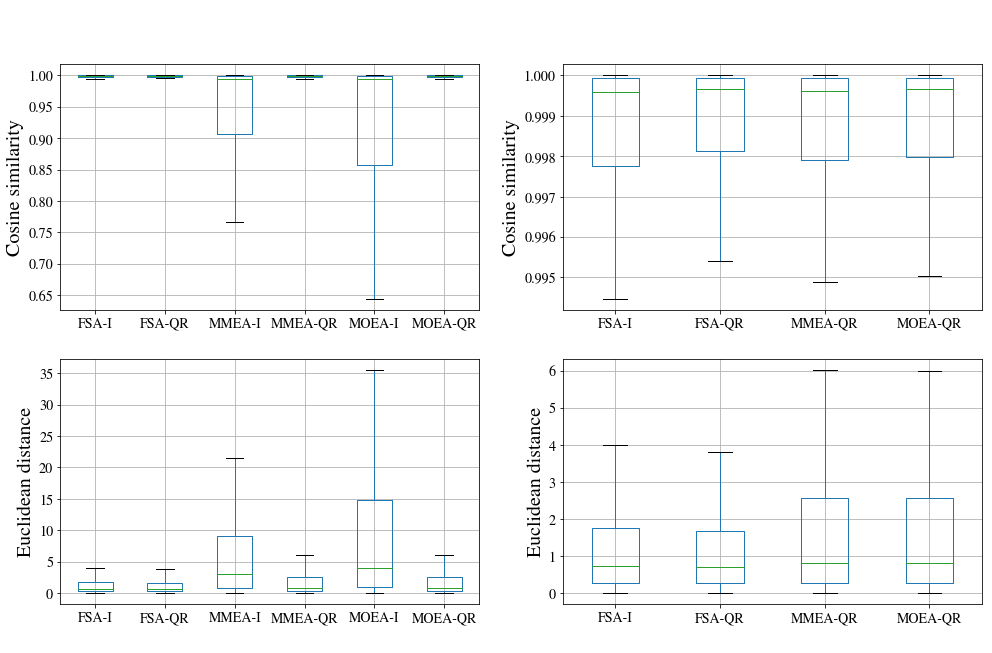
\includegraphics[width=14cm]{img/all_distances_feasible}

    \caption{Similarity of the solutions given by the algorithms finding $h$-element subsets satisfying strong necessary condition compared to the OLS solution on the subset of the data set that does not contain outliers. On the left are two box plots for all algorithms. Since visualization is influenced by the scale of MMEA-I and MOEA-I box plots, we provide two graphs without these two algorithms on the right.}
    \label{all_distances}
\end{figure}

\subsection{Algorithms for finding exact solution}
Here we provide results of the algorithms finding the exact solution. For the improved versions of the BAB and BSA algorithms, which can utilize results of appropriate solution we decided to use solutions given by the FSA-QR. This algorithm, as observed in previous section, provide the best results. FSA-QR is quite slow compared to the MOEA and MMEA variations, but because exact algorithms have much higher time complexity (thus can be used only on very small data sets), we do not sacrifice any speed performance.

The setup for the simulations is the same as in previous section but we only compare speed this time, because all of the algorithms provide exact solution. 

The results are given in Appendix~\ref{apendix:strong} in Tables~\ref{table1}, \ref{table2} and \ref{table3} for data sets $D1$, $D2$ and $D3$ respectively. 
    
We can see that 
